\linespread{1.6}\selectfont

\section{Results}

\subsection{1-D model}

\begin{figure}[here]
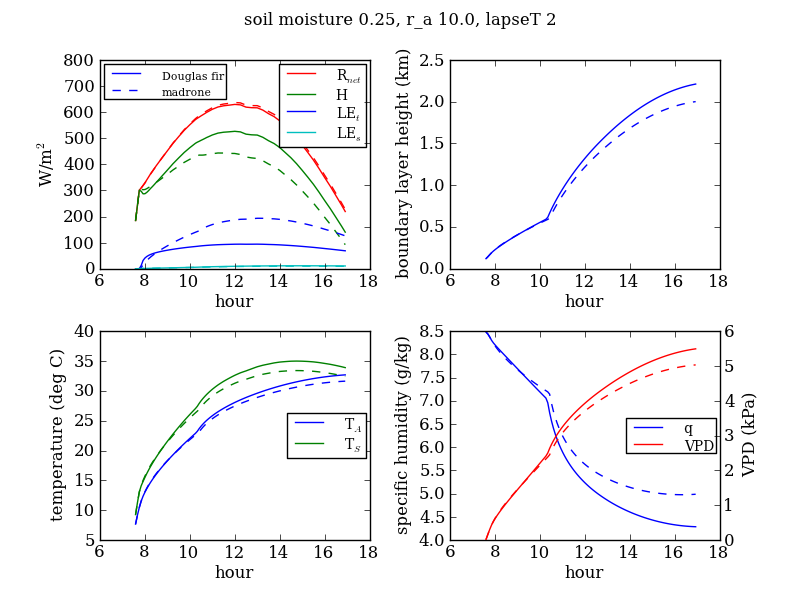
\includegraphics[width=1\textwidth]{ch2-BL/figures/testall_Aug15_soilm0pt25_ra10_lapseT2.png}
\caption{}
\label{fig:BL_1Ddiurnal}
\end{figure}

The 1-D model simulates a reasonable diurnal cycle, but with temperatures several degrees higher than observations.  Figure \ref{fig:BL_1Ddiurnal} shows a typical diurnal cycle for lapse rate 2 and relative soil moisture ($\theta_{rel}$) $= 0.25$.  The model run with a Pacific madrone forest has higher transpiration than the run with a Douglas fir forest, because Pacific madrone stomatal conductance is higher at this value of $\theta_{rel}$ (c.f. Figure XX); both cases have very little soil evaporation at this value of $\theta_{rel}$.  As a result, the Pacific madrone case has lower $H$, lower $h$, lower $T_s$ and $T_a$, and higher $Q$ than the Douglas fir case.

\begin{figure}[here]
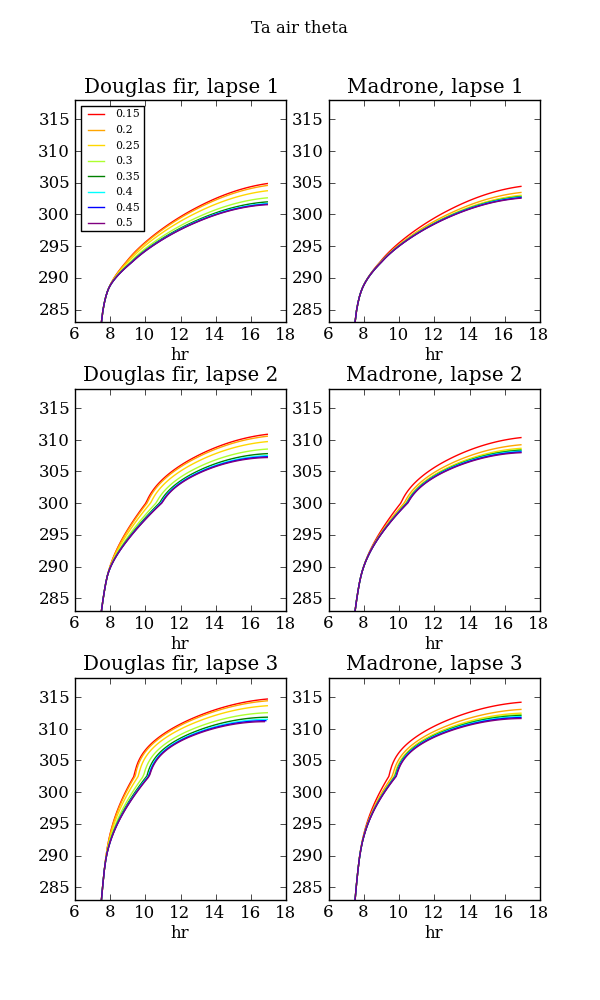
\includegraphics[width=0.5\textwidth]{ch2-BL/figures/testall_compare_sm_lapse_Ta.png}
\caption{}
\label{fig:BL_1DdiurnalTa}
\end{figure}

\begin{figure}[here]
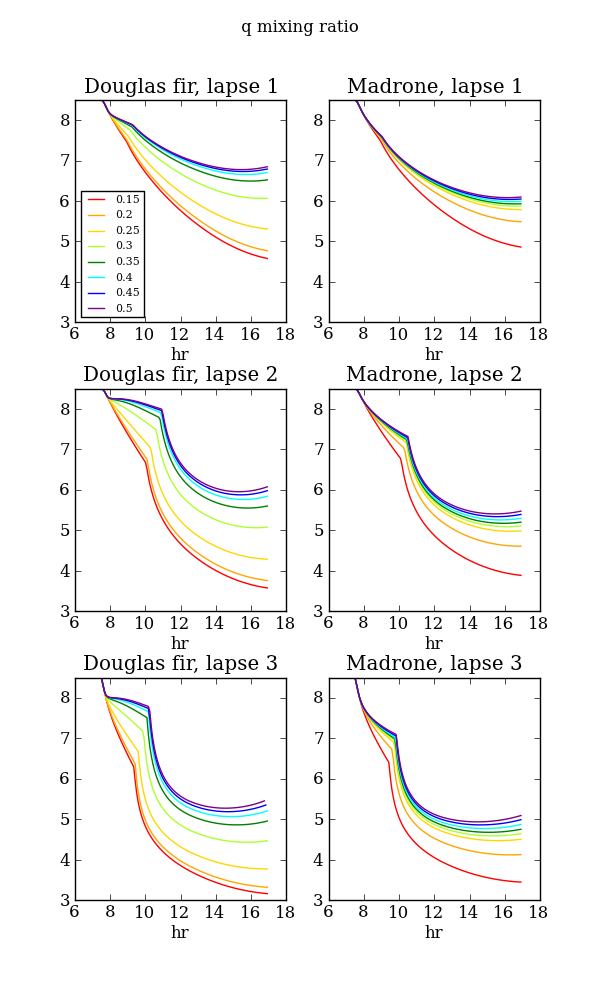
\includegraphics[width=0.5\textwidth]{ch2-BL/figures/testall_compare_sm_lapse_q.png}
\caption{}
\label{fig:BL_1DdiurnalQ}
\end{figure}

%\clearpage

Figures \ref{fig:BL_1DdiurnalTa} and \ref{fig:BL_1DdiurnalQ} show the dependence of diurnal cycles of $T_a$ and $Q$ on $\theta_{rel}$ and free troposphere conditions.  For both the Pacific madrone case and the Douglas fir case, decreasing $\theta_{rel}$ leads to increasing $T_a$ and decreasing $Q$.  However, the increase in $T_a$ and decrease in $Q$ begin at higher (wetter) values of $\theta_{rel}$ in the Douglas fir case than in the Pacific madrone case.  As expected, the hotter free troposphere conditions resulted in higher $T_a$ (increasing $T_a$ from lapse rate 1 to 2 to 3).  Additionally, the shape of the diurnal cycle differed among the free troposphere cases, with $T_a$ rising most rapidly in the morning for the hottest case (lapse rate 3), resulting from entrainment of high-$\Theta$ air in the steep inversion.  The hotter free troposphere conditions also led to lower $Q$, but with a slower morning decline of $Q$ because of relatively slow boundary layer growth through the steep inversion.

\begin{figure}[here]
\begin{subfigure}{0.5\textwidth}
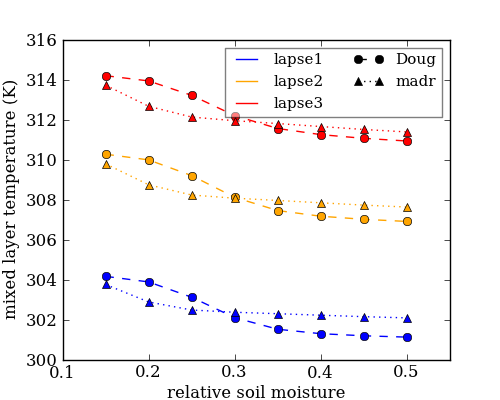
\includegraphics[width=\textwidth]{ch2-BL/figures/all_afternoon_T.png}
\caption{}
\end{subfigure}
\begin{subfigure}{0.5\textwidth}
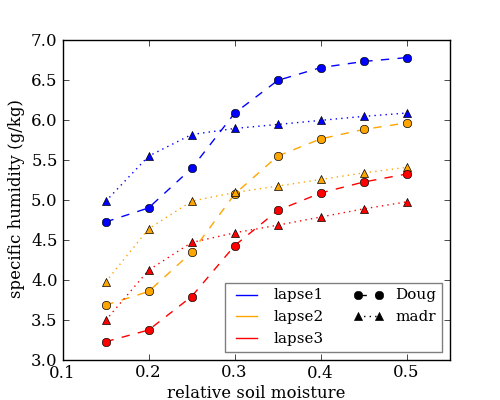
\includegraphics[width=\textwidth]{ch2-BL/figures/all_afternoon_Q.png}
\caption{}
\end{subfigure}
\caption{}
\label{fig:BL_345changes}
\end{figure}

%\clearpage

The differences between the species cases are largest in the afternoon; Figure \ref{fig:BL_345changes} illustrates the differences at 3:45 pm in $T_a$ and $Q$ between the Douglas fir and Pacific madrone cases, as a function of $\theta_{rel}$ and free troposphere conditions.  The differences between the Douglas fir and Pacific madrone cases for both $T_a$ and $Q$ are largest at $\theta_{rel}$ values around 0.2, with the Douglas fir case hotter by XX $^o$C and drier by XX g/kg.  A $\theta_{rel}$ value of 0.2-0.25 is typical for the mid- to late-dry-season at the ACRR [\textit{Link et al.}, 2013].  The differences in $T_a$ and $Q$ are somewhat larger for the hottest free troposphere conditions (lapse rate 3).  Interestingly, at $\theta_{rel}$ values higher than about 0.35, the Douglas fir case is actually cooler and moister; such $\theta_{rel}$ values are typical for the late spring and early summer at the ACRR [\textit{Link et al.}, 2013].

%- fraction of moisture from land surface vs. from free troposphere, for different soil moisture / lapse rate / species conditions

\subsection{Regional climate model}
The regional climate model simulates similar temperature and humidity differences as the 1-D model.  Mid-afternoon (XX pm) temperature is warmer in the Douglas-fir case than in the Pacific madrone case by RANGE $^o$C, with the highest temperature difference for an assigned soil moisture of XX (Figure XX); the difference in mid-afternoon is largest at the model level nearest the surface (XX $^o$C) but extends through the lower XX m of the atmosphere with smaller magnitude (XX $^o$C).  Coastal areas in the experimental region (within XX km of the ocean) show a smaller difference between the species cases away from the surface (model levels greater than XX).  There is some downwind transport of the warmer air from the experimental region, especially between 4 pm and 10 pm, when the lower atmosphere over the northern Central Valley is up to XX degrees warmer in the Douglas-fir case than in the Pacific madrone case.

The Douglas-fir case also has lower mid-afternoon specific humidity than the Pacific madrone case water vapor by $\sim$ XX g/kg (Figure XX, top row); again, the difference is largest at an imposed soil moisture value of XX and extends throughout the boundary layer (model layers XX).  The difference is largest in the afternoon and evening (XX pm to XX pm, XX g/kg).  There is again some advection of the drier air (XX g/kg drier in the Douglas-fir case) to the northern Central Valley in the afternoon and evening (XX pm to XX pm).

The hotter and drier boundary layer in the Douglas-fir simulations result from suppressed transpiration and increased sensible heat flux in the Douglas fir case (Figure XX), arising from the greater Douglas-fir stomatal sensitivity to dry soils.   Douglas-fir latent heat flux at 4 pm local time was lower than Pacific madrone transpiration by XX to XX W/m$^2$, and sensible heat flux was higher in the Douglas-fir case by XX to XX W/m$^2$.  The higher sensible heat flux drives greater growth of boundary layer (Figure XX, bottom row), leading to more entrainment of hot, dry free troposphere air.


